\section{Design}

\subsection{System Architecture Diagrams}

\subsubsection{Component-Level Architecture}

The system is composed of four hardware-connected components and one host interface, all orchestrated by the Arduino Mega 2560 microcontroller. The serial terminal running on the host PC provides the command-input path over the USB-to-UART bridge; the red LED on digital pin D7 acts as the binary actuator output (simulating a relay or solenoid); and the 16x2 I2C LCD provides continuous visual feedback. All components share a common ground and the 5\,V supply provided by the board's voltage regulator. The bidirectional data flow between the PC and the MCU is achieved through UART0 at 9600 baud: the user types \texttt{ON} or \texttt{OFF} commands that travel from the terminal to the MCU, while status confirmation messages and periodic structured reports travel from the MCU back to the terminal.

\begin{figure}[H]
\centering
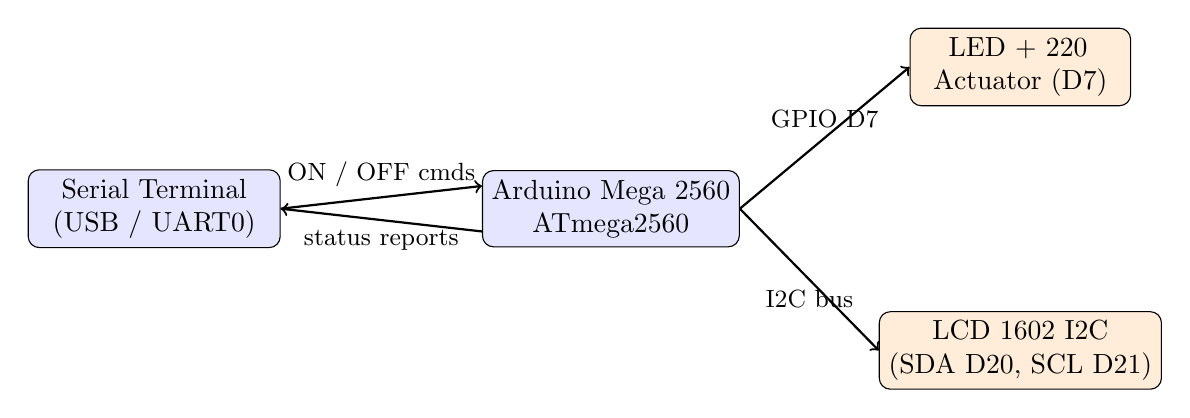
\begin{tikzpicture}[
    comp/.style={draw, rectangle, rounded corners, minimum width=3.2cm,
                 minimum height=0.9cm, text centered, align=center, fill=blue!10},
    hw/.style={draw, rectangle, rounded corners, minimum width=2.8cm,
               minimum height=0.9cm, text centered, align=center, fill=orange!15}
]
    \node[comp] (mcu)    at (0,    0)    {Arduino Mega 2560\\ATmega2560};
    \node[comp] (pc)     at (-5.8,  0)   {Serial Terminal\\(USB / UART0)};
    \node[hw]   (led)    at ( 5.2,  1.8) {LED + 220\,\si{\ohm}\\Actuator (D7)};
    \node[hw]   (lcd)    at ( 5.2, -1.8) {LCD 1602 I2C\\(SDA D20, SCL D21)};

    \draw[->, thick] (pc.east) -- node[above, font=\small]{ON / OFF cmds} (mcu.170);
    \draw[<-, thick] (pc.east) -- node[below, font=\small]{status reports} (mcu.190);
    \draw[->, thick] (mcu.east) -- node[above, font=\small]{GPIO D7} (led.west);
    \draw[->, thick] (mcu.east) -- node[below, font=\small]{I2C bus} (lcd.west);
\end{tikzpicture}
\caption{System component-level architecture for Lab 4.1}
\label{fig:system_component_diagram}
\end{figure}

The component diagram shows that the Arduino Mega 2560 is the central hub of the system. The serial terminal is the sole input source: the user types a command and the microcontroller's UART0 receive register captures the bytes. After parsing and conditioning, the output path branches into two: the GPIO output toggles the actuator LED, and the I2C output updates the LCD display. This simple fan-out topology is characteristic of small embedded control systems where a single processor manages all peripherals without external bus arbitration or multi-master contention.

\subsubsection{Layered System Architecture}

The software is organized into five layers following the automotive-inspired AUTOSAR-like layered architecture used consistently throughout the lab series. Each layer communicates exclusively with its immediate neighbours through well-defined header-file interfaces. This strict layering ensures that changes to one layer (for example, replacing the LED with a relay module) propagate only to the layer directly above or below.

\begin{figure}[H]
\centering
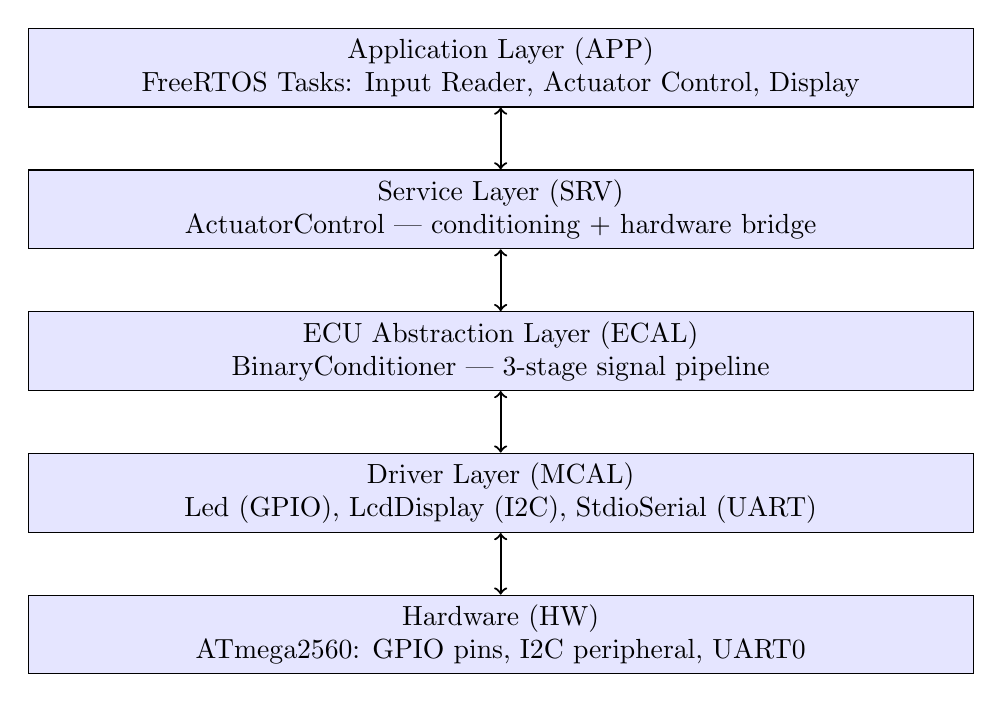
\begin{tikzpicture}[
    box/.style={draw, rectangle, minimum width=12cm, minimum height=1.0cm,
                text centered, align=center, fill=blue!10},
    node distance=0.5cm]
    \node[box] (app)  at (0, 0)     {Application Layer (APP)\\FreeRTOS Tasks: Input Reader, Actuator Control, Display};
    \node[box] (srv)  at (0, -1.8)  {Service Layer (SRV)\\ActuatorControl — conditioning + hardware bridge};
    \node[box] (ecal) at (0, -3.6)  {ECU Abstraction Layer (ECAL)\\BinaryConditioner — 3-stage signal pipeline};
    \node[box] (mcal) at (0, -5.4)  {Driver Layer (MCAL)\\Led (GPIO), LcdDisplay (I2C), StdioSerial (UART)};
    \node[box] (hw)   at (0, -7.2)  {Hardware (HW)\\ATmega2560: GPIO pins, I2C peripheral, UART0};
    \foreach \a/\b in {app/srv, srv/ecal, ecal/mcal, mcal/hw}
        \draw[<->, thick] (\a) -- (\b);
\end{tikzpicture}
\caption{Layered software architecture of the Lab 4.1 system}
\label{fig:layered_architecture}
\end{figure}

The \textbf{Hardware (HW)} layer consists of the physical ATmega2560 microcontroller with its GPIO peripheral (pin D7 driving the actuator LED), the TWI/I2C peripheral (pins D20/D21 driving the LCD backpack), and the UART0 peripheral (connected to USB for host communication).

The \textbf{Driver Layer (MCAL)} contains three reusable library modules. The \texttt{Led} class encapsulates all \texttt{pinMode()} and \texttt{digitalWrite()} calls behind a clean API of \texttt{init()}, \texttt{turnOn()}, \texttt{turnOff()}, \texttt{toggle()}, and \texttt{isOn()} methods. The \texttt{LcdDisplay} class wraps the \texttt{LiquidCrystal\_I2C} library into a line-based display interface with automatic padding. The \texttt{StdioSerial} module redirects the C standard I/O streams to UART0 using \texttt{fdev\_setup\_stream()}.

The \textbf{ECU Abstraction Layer (ECAL)} contains the \texttt{BinaryConditioner} class, which implements the three-stage signal conditioning pipeline (saturation, debouncing, persistent validation) in a purely software domain, operating entirely on boolean values with no hardware knowledge.

The \textbf{Service Layer (SRV)} contains \texttt{ActuatorControl}, which wires the \texttt{BinaryConditioner} to the \texttt{Led} driver. It accepts raw ON/OFF commands, processes them through the conditioner, and updates the hardware only when the conditioned state changes.

The \textbf{Application Layer (APP)} consists of the three FreeRTOS tasks and the shared state structure (\texttt{ActuatorShared}) that orchestrate the overall system behaviour.

\subsection{Block Diagrams}

\subsubsection{System Data Flow and FreeRTOS Task Architecture}

The three FreeRTOS tasks communicate through a mutex-protected shared structure \texttt{g\_actuator}. The diagram below illustrates the data-flow direction between tasks and the shared memory, as well as the period and priority of each task. Task 1 (Input Reader) is the highest-priority task because it must respond to serial input within one polling interval (10\,ms). Task 2 (Actuator Control) runs at medium priority to process the conditioning pipeline every 75\,ms. Task 3 (Display/Report) runs at the lowest priority since display updates are the least time-sensitive operation.

\begin{figure}[H]
\centering
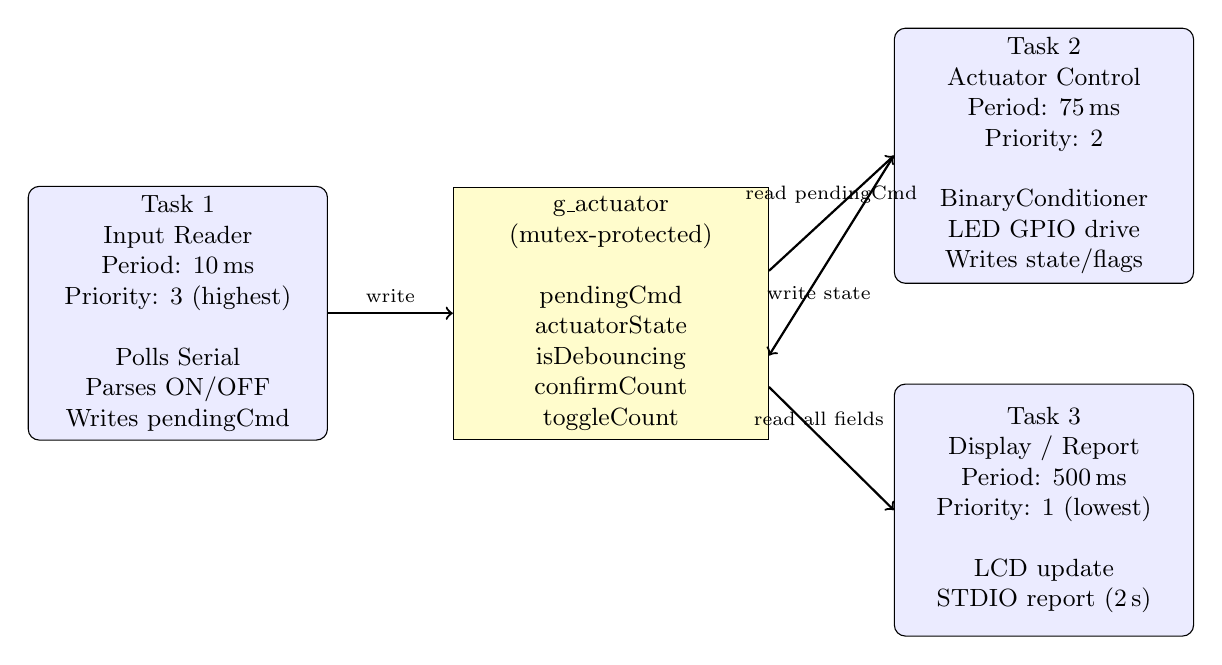
\begin{tikzpicture}[
    task/.style={draw, rectangle, rounded corners, minimum width=3.8cm,
                 minimum height=3.2cm, text centered, align=center, fill=blue!8,
                 font=\small},
    shared/.style={draw, rectangle, minimum width=4.0cm, minimum height=1.6cm,
                   text centered, align=center, fill=yellow!20, font=\small}
]
    \node[task] (t1) at (-5.5, 0) {Task 1\\Input Reader\\Period: 10\,ms\\Priority: 3 (highest)\\\\Polls Serial\\Parses ON/OFF\\Writes pendingCmd};

    \node[shared] (sh) at (0, 0) {g\_actuator\\(mutex-protected)\\\\pendingCmd\\actuatorState\\isDebouncing\\confirmCount\\toggleCount};

    \node[task] (t2) at (5.5, 2.0) {Task 2\\Actuator Control\\Period: 75\,ms\\Priority: 2\\\\BinaryConditioner\\LED GPIO drive\\Writes state/flags};

    \node[task] (t3) at (5.5, -2.5) {Task 3\\Display / Report\\Period: 500\,ms\\Priority: 1 (lowest)\\\\LCD update\\STDIO report (2\,s)};

    \draw[->, thick] (t1.east) -- node[above, font=\scriptsize]{write} (sh.west);
    \draw[->, thick] (sh.15)   -- node[above, font=\scriptsize]{read pendingCmd} (t2.west);
    \draw[->, thick] (t2.west) -- node[below, font=\scriptsize, pos=0.6]{write state} (sh.345);
    \draw[->, thick] (sh.335)  -- node[above, font=\scriptsize, pos=0.4]{read all fields} (t3.west);
\end{tikzpicture}
\caption{FreeRTOS task data-flow diagram for Lab 4.1}
\label{fig:task_dataflow}
\end{figure}

The shared structure uses a FreeRTOS mutex (\texttt{xSemaphoreCreateMutex()}) to prevent data races. Every read or write to the shared fields is bracketed by \texttt{xSemaphoreTake()} and \texttt{xSemaphoreGive()} calls with a 5--10\,ms timeout. The short timeout ensures that if one task is delayed, the others are not blocked indefinitely. In practice, the critical sections are short (a few microseconds for reading/writing primitive fields), so mutex contention is negligible.

\subsubsection{Input Reader Task Flowchart}

The input reader task polls the hardware serial port at 10\,ms intervals. Incoming characters are accumulated into a line buffer with local echo. When a newline is received, the buffer is trimmed and uppercased, then matched against the known commands \texttt{ON} and \texttt{OFF}. Valid commands are written to \texttt{g\_actuator.pendingCmd} under mutex protection; unrecognized input is rejected with an error message.

\tikzset{
    startstop/.style={rectangle, rounded corners, minimum width=3.0cm,
        minimum height=0.75cm, text centered, align=center, draw=black, fill=gray!15},
    process/.style={rectangle, minimum width=3.0cm,
        minimum height=0.75cm, text centered, align=center, draw=black, fill=blue!10},
    decision/.style={diamond, aspect=2.5, minimum width=2.5cm,
        minimum height=0.75cm, text centered, align=center, draw=black, fill=orange!15},
    io/.style={trapezium, trapezium left angle=70, trapezium right angle=110,
        minimum width=3.0cm, minimum height=0.75cm, text centered, align=center,
        draw=black, fill=green!10},
    arrow/.style={thick,->,>=Stealth}
}

\begin{figure}[H]
\centering
\begin{tikzpicture}
    \node (start)  [startstop] at (0,  0.0)   {vTaskInputReader};
    \node (prompt) [process]   at (0, -1.8)   {Print prompt ``$>$ ''};
    \node (loop)   [startstop] at (0, -3.6)   {Polling loop};
    \node (d1)     [decision]  at (0, -6.1)   {Serial.\\available()?};
    \node (read)   [process]   at (4.5, -6.1) {Read char c\\echo to terminal};
    \node (d2)     [decision]  at (4.5, -9.0) {c == newline?};
    \node (buf)    [process]   at (8.0, -9.0) {Append c\\to buf[len++]};
    \node (norm)   [process]   at (4.5,-11.8) {Trim \& uppercase\\normalizeInput(buf)};
    \node (d3)     [decision]  at (4.5,-14.5) {buf ==\\``ON'' or ``OFF''?};
    \node (write)  [process]   at (4.5,-17.0) {Take mutex\\write pendingCmd\\give mutex};
    \node (err)    [process]   at (9.0,-14.5) {Print error\\``Unknown cmd''};
    \node (reset)  [process]   at (4.5,-19.0) {len = 0\\print ``$>$ ''};
    \node (delay)  [process]   at (0, -8.8)   {vTaskDelayUntil\\10\,ms};

    \draw [arrow] (start)  -- (prompt);
    \draw [arrow] (prompt) -- (loop);
    \draw [arrow] (loop)   -- (d1);
    \draw [arrow] (d1)     -- node[above]{\small Yes} (read);
    \draw [arrow] (d1)     -- node[left]{\small No}   (delay);
    \draw [arrow] (delay.west) -- ++(-1.8,0) |- (loop.west);
    \draw [arrow] (read)   -- (d2);
    \draw [arrow] (d2)     -- node[above]{\small No}  (buf);
    \draw [arrow] (buf.north) -- ++(0, 0.5) -| (4.5, -6.1) -- (read.south);
    \draw [arrow] (d2)     -- node[right]{\small Yes} (norm);
    \draw [arrow] (norm)   -- (d3);
    \draw [arrow] (d3)     -- node[right]{\small Yes} (write);
    \draw [arrow] (d3)     -- node[above]{\small No}  (err);
    \draw [arrow] (write)  -- (reset);
    \draw [arrow] (err.south) -- ++(0,-1.0) -| (reset.east);
    \draw [arrow] (reset.west) -- ++(-4.5, 0) |- (loop.west);
\end{tikzpicture}
\caption{Flowchart of the Input Reader task (\texttt{vTaskInputReader})}
\label{fig:task_input_flowchart}
\end{figure}

\subsubsection{BinaryConditioner Pipeline Flowchart}

The \texttt{BinaryConditioner::process()} function is the heart of the signal conditioning pipeline. It is called once per Actuator Control task tick (every 75\,ms) with the current raw command. The three stages — saturation, debouncing, and persistent validation — are evaluated in sequence. A state transition is committed to the conditioned output only when \emph{both} the debounce timer has elapsed \emph{and} the required number of consecutive identical samples has been reached.

\begin{figure}[H]
\centering
\begin{tikzpicture}
    \node (start)   [startstop] at (0,    0.0)  {process(rawInput)};
    \node (sat)     [process]   at (0,   -1.8)  {Stage 1: Saturate\\saturated = rawInput ? true : false};
    \node (d1)      [decision]  at (0,   -4.8)  {saturated ==\\pendingState?};
    \node (restart) [process]   at (-5.0, -4.8) {Restart debounce:\\pending = saturated\\startMs = millis()\\confirm = 1};
    \node (d2)      [decision]  at (0,   -8.0)  {pending !=\\conditioned?};
    \node (incr)    [process]   at (4.5,  -8.0) {confirmCount++};
    \node (d3)      [decision]  at (0,  -11.2)  {count $\geq$ N\\AND elapsed\\$\geq$ Tms?};
    \node (commit)  [process]   at (0,  -14.2)  {Commit transition:\\conditioned = pending\\debounce = false\\confirmCount = 0};
    \node (stable)  [process]   at (4.5, -11.2) {inDebounce = false};
    \node (ret)     [startstop] at (0,  -16.2)  {return conditioned};

    \draw [arrow] (start)   -- (sat);
    \draw [arrow] (sat)     -- (d1);
    \draw [arrow] (d1)      -- node[above, font=\small]{No} (restart);
    \draw [arrow] (d1)      -- node[right, font=\small]{Yes} (d2);
    % Route restart back to d2 via the LEFT side, avoiding d1
    \draw [arrow] (restart.south) -- ++(0,-0.8) -- (-5.0,-6.6) -- (-2.5,-6.6) -- (-2.5,-7.3) -- (d2.west);
    \draw [arrow] (d2)      -- node[above, font=\small]{Yes} (incr);
    % Route incr down to d3 via right side
    \draw [arrow] (incr.south) -- ++(0,-0.6) -- (2.5,-9.6) -- (2.5,-10.4) -- (d3.east);
    \draw [arrow] (d2)      -- node[right, font=\small, pos=0.4]{No (pending==conditioned)} (d3);
    \draw [arrow] (d3)      -- node[right, font=\small]{Yes} (commit);
    \draw [arrow] (d3)      -- node[above, font=\small]{No} (stable);
    \draw [arrow] (stable.south) -- ++(0,-2.5) -| (ret.east);
    \draw [arrow] (commit)  -- (ret);
\end{tikzpicture}
\caption{Flowchart of \texttt{BinaryConditioner::process()} --- 3-stage signal conditioning}
\label{fig:conditioner_flowchart}
\end{figure}

The critical design decision visible in this flowchart is the dual guard on state commitment: both the debounce timer (Stage 2) and the persistence counter (Stage 3) must be satisfied simultaneously. If the input oscillates rapidly, the persistence counter resets before reaching N, blocking the transition even if the debounce window has elapsed. Conversely, if the input stabilizes instantly after a change but then reverts before the debounce window expires, the transition is still blocked. This makes the conditioner robust against both periodic glitches and burst noise.

\subsubsection{Actuator Control Task Flowchart}

The Actuator Control task runs at 75\,ms. On each tick it reads the pending command from the shared state, passes it through the \texttt{ActuatorControl::update()} method (which internally invokes \texttt{BinaryConditioner::process()} and drives the LED), and writes the resulting conditioned state back to the shared memory.

\begin{figure}[H]
\centering
\begin{tikzpicture}
    \node (start)  [startstop] at (0,  0.0)  {vTaskActuator starts};
    \node (init)   [process]   at (0, -1.8)  {s\_actuator.init()\\LED pin = OUTPUT, state = OFF};
    \node (loop)   [startstop] at (0, -3.6)  {Periodic task loop};
    \node (read)   [process]   at (0, -5.6)  {xSemaphoreTake(mutex)\\rawCmd = g\_actuator.pendingCmd\\xSemaphoreGive(mutex)};
    \node (set)    [process]   at (0, -7.8)  {s\_actuator.setRawCommand(rawCmd)};
    \node (upd)    [process]   at (0, -9.6)  {s\_actuator.update()\\(runs BinaryConditioner +\\drives LED GPIO)};
    \node (write)  [process]   at (0,-11.8)  {xSemaphoreTake(mutex)\\write actuatorState, isDebouncing\\confirmCount, toggleCount\\xSemaphoreGive(mutex)};
    \node (delay)  [process]   at (0,-14.2)  {vTaskDelayUntil(75\,ms)};

    \draw [arrow] (start) -- (init);
    \draw [arrow] (init)  -- (loop);
    \draw [arrow] (loop)  -- (read);
    \draw [arrow] (read)  -- (set);
    \draw [arrow] (set)   -- (upd);
    \draw [arrow] (upd)   -- (write);
    \draw [arrow] (write) -- (delay);
    \draw [arrow] (delay.west) -- ++(-2.5,0) |- (loop.west);
\end{tikzpicture}
\caption{Flowchart of the Actuator Control task (\texttt{vTaskActuator})}
\label{fig:task_actuator_flowchart}
\end{figure}

\subsubsection{Display and Reporting Task Flowchart}

The Display task runs at 500\,ms. It reads the complete shared state under mutex protection, formats and displays the actuator status on the I2C LCD, and every four ticks (approximately every 2 seconds) prints a structured report to the serial terminal via \texttt{printf()}.

\begin{figure}[H]
\centering
\begin{tikzpicture}
    \node (start)  [startstop] at (0,  0.0)  {vTaskDisplay starts};
    \node (init)   [process]   at (0, -1.8)  {s\_lcd.init()\\Show ``Actuator Ctrl'' / ``Initializing...''};
    \node (loop)   [startstop] at (0, -3.6)  {Periodic task loop};
    \node (read)   [process]   at (0, -5.8)  {xSemaphoreTake(mutex)\\Read: state, rawCmd,\\debouncing, confirmCnt, toggleCnt\\xSemaphoreGive(mutex)};
    \node (lcd)    [process]   at (0, -8.2)  {Update LCD:\\Line 1: ``Actuator: ON'' / ``OFF''\\Line 2: ``STABLE'' / ``DEBOUNCING''};
    \node (d1)     [decision]  at (0,-11.0)  {tick $\geq$\\REPORT\_N?};
    \node (rpt)    [process]   at (-4.5,-11.0) {printf structured\\STDIO report\\tick = 0};
    \node (delay)  [process]   at (0,-13.5)  {tick++\\vTaskDelayUntil(500\,ms)};

    \draw [arrow] (start) -- (init);
    \draw [arrow] (init)  -- (loop);
    \draw [arrow] (loop)  -- (read);
    \draw [arrow] (read)  -- (lcd);
    \draw [arrow] (lcd)   -- (d1);
    \draw [arrow] (d1)    -- node[above]{\small Yes} (rpt);
    \draw [arrow] (d1)    -- node[right]{\small No}  (delay);
    \draw [arrow] (rpt.south) -- ++(0,-0.5) -| (delay.west);
    \draw [arrow] (delay.west) -- ++(-2.5,0) |- (loop.west);
\end{tikzpicture}
\caption{Flowchart of the Display and Reporting task (\texttt{vTaskDisplay})}
\label{fig:task_display_flowchart}
\end{figure}

\subsubsection{ActuatorControl::update() Flowchart}

The \texttt{update()} method in the \texttt{ActuatorControl} service layer converts the raw command to a boolean, passes it through the \texttt{BinaryConditioner::process()} pipeline, and conditionally updates the hardware LED. The GPIO output is only toggled when the conditioned state actually changes, avoiding unnecessary \texttt{digitalWrite()} calls on every tick.

\begin{figure}[H]
\centering
\begin{tikzpicture}
    \node (start)  [startstop] at (0,  0.0)  {update()};
    \node (conv)   [process]   at (0, -1.8)  {rawBool = (\_rawCommand == ON)};
    \node (cond)   [process]   at (0, -3.6)  {conditioned = \_conditioner.process(rawBool)};
    \node (map)    [process]   at (0, -5.4)  {newState = conditioned ? ON : OFF};
    \node (d1)     [decision]  at (0, -8.0)  {newState !=\\\_currentState?};
    \node (apply)  [process]   at (0,-10.5)  {\_currentState = newState\\if ON: \_led.turnOn()\\else: \_led.turnOff()};
    \node (ret)    [startstop] at (0,-12.5)  {return};

    \draw [arrow] (start) -- (conv);
    \draw [arrow] (conv)  -- (cond);
    \draw [arrow] (cond)  -- (map);
    \draw [arrow] (map)   -- (d1);
    \draw [arrow] (d1)    -- node[right]{\small Yes} (apply);
    \draw [arrow] (d1.east) -- ++(2.5,0) |- node[right, pos=0.3]{\small No} (ret.east);
    \draw [arrow] (apply) -- (ret);
\end{tikzpicture}
\caption{Flowchart of \texttt{ActuatorControl::update()}}
\label{fig:actuator_update_flowchart}
\end{figure}

\subsection{Electrical Schematics}

\subsubsection{Component Specification}

The circuit uses three components beyond the Arduino Mega 2560 development board itself:

\begin{enumerate}
    \item \textbf{Red LED (5\,mm)}: The binary actuator output on pin D7. Forward voltage: approximately 2.0\,V. Maximum forward current: 20\,mA. The LED simulates a real-world binary actuator such as a relay coil or solenoid driver.

    \item \textbf{220\,\si{\ohm} Resistor}: Connected in series with the LED to limit current. With a 5\,V supply and a 2.0\,V LED forward voltage, the current is $I = (5.0 - 2.0) / 220 \approx 13.6$\,mA, which is safely below the 20\,mA maximum and the ATmega2560's 20\,mA per-pin GPIO current limit.

    \item \textbf{LCD 1602 I2C Module}: A 16-column, 2-row character LCD with a PCF8574 I2C backpack. The module is powered from the 5\,V rail and communicates over the I2C bus using the standard 7-bit address 0x27. The SDA and SCL lines are connected to the Mega's dedicated I2C pins (D20 and D21 respectively). Internal pull-up resistors on the backpack module eliminate the need for external I2C pull-ups.
\end{enumerate}

\subsubsection{Circuit Connections}

The electrical connections are illustrated in the schematic below. The LED branch forms a simple series path: pin D7 sources current through the 220\,\si{\ohm} resistor and the LED to ground. The I2C LCD requires four connections: VCC (5\,V), GND, SDA (D20), and SCL (D21).

\begin{figure}[H]
\centering
\begin{circuitikz}[scale=0.9, transform shape]
    % Actuator LED branch
    \draw (0, 0) node[anchor=east]{\small Arduino Pin D7}
        to[R, l=220\,\si{\ohm}, o-] (3.5, 0)
        to[leD*, color=red, l_={\small Red LED}] (5.5, 0)
        node[ground] {};

    % Separator
    \draw[dashed, gray] (-1.5, -1.0) -- (6.0, -1.0);

    % I2C LCD connections
    \node[anchor=east] at (0, -1.8) {\small SDA (Pin D20)};
    \draw[-] (0, -1.8) -- (5.5, -1.8) node[anchor=west]{\small LCD SDA};
    \node[anchor=east] at (0, -2.6) {\small SCL (Pin D21)};
    \draw[-] (0, -2.6) -- (5.5, -2.6) node[anchor=west]{\small LCD SCL};
    \node[anchor=east] at (0, -3.4) {\small 5\,V};
    \draw[-] (0, -3.4) -- (5.5, -3.4) node[anchor=west]{\small LCD VCC};
    \node[anchor=east] at (0, -4.2) {\small GND};
    \draw[-] (0, -4.2) -- (5.5, -4.2) node[anchor=west]{\small LCD GND};
\end{circuitikz}
\caption{Electrical schematic for Lab 4.1 — actuator LED circuit and I2C LCD connections}
\label{fig:electrical_schematic}
\end{figure}

\subsubsection{Pin Mapping Summary}

\begin{table}[H]
\centering
\caption{Pin mapping for Lab 4.1}
\label{tab:pin_mapping}
\begin{tabular}{|l|l|l|}
\hline
\textbf{Arduino Pin} & \textbf{Component} & \textbf{Function} \\
\hline
D7  & Red LED (via 220\,\si{\ohm}) & Binary actuator output \\
D20 (SDA) & LCD 1602 I2C backpack & I2C data line \\
D21 (SCL) & LCD 1602 I2C backpack & I2C clock line \\
USB (UART0) & Host PC serial terminal & Command input / status output \\
5V  & LCD module VCC & Power supply \\
GND & LED cathode, LCD GND & Common ground \\
\hline
\end{tabular}
\end{table}

\subsubsection{Hardware Configuration}

The complete Wokwi simulation is defined in \texttt{labs/wokwi/lab4.1/diagram.json} and loaded via \texttt{wokwi.toml}. The configuration below lists all virtual components and their wire connections.

\begin{lstlisting}[language=json, caption=Wokwi hardware configuration (\texttt{diagram.json}), label=lst:wokwi_json]
{
  "version": 1,
  "author": "Vremere Adrian",
  "editor": "wokwi",
  "parts": [
    { "type": "wokwi-arduino-mega", "id": "mega",
      "top": 0, "left": 0 },
    { "type": "wokwi-lcd1602",      "id": "lcd1",
      "top": -320, "left": 100,
      "attrs": { "pins": "i2c" } },
    { "type": "wokwi-led",          "id": "led_act",
      "top": 280, "left": 220,
      "attrs": { "color": "red", "label": "Actuator" } },
    { "type": "wokwi-resistor",     "id": "r_act",
      "top": 245, "left": 200, "rotate": 90,
      "attrs": { "resistance": "220" } }
  ],
  "connections": [
    ["lcd1:VCC", "mega:5V",    "red",
      ["v20", "h-60", "v200"]],
    ["lcd1:GND", "mega:GND.1", "black",
      ["v20", "h-40", "v200"]],
    ["lcd1:SDA", "mega:20",    "cyan",
      ["v40", "h100", "v140"]],
    ["lcd1:SCL", "mega:21",    "darkgreen",
      ["v60", "h120", "v120"]],
    ["mega:7",     "r_act:1",    "orange",
      ["v60", "h0", "v80"]],
    ["r_act:2",    "led_act:A",  "orange",  ["v0"]],
    ["led_act:C",  "mega:GND.2", "black",
      ["v30", "h-160", "v-200"]]
  ]
}
\end{lstlisting}

The \texttt{wokwi.toml} file configures the Wokwi VS Code extension to load the compiled firmware directly from the PlatformIO build output directory:

\begin{lstlisting}[caption=Wokwi firmware configuration (\texttt{wokwi.toml}), label=lst:wokwi_toml]
[wokwi]
version = 1
firmware = "../../.pio/build/lab4_1/firmware.hex"
elf = "../../.pio/build/lab4_1/firmware.elf"
\end{lstlisting}

\begin{figure}[H]
\centering
\IfFileExists{resources/Design/ElectricalSchematics/wokwi_circuit.png}{%
    
\includegraphics[width=0.85\textwidth]{resources/Design/ElectricalSchematics/wokwi_circuit.png}%
}{%
    \fbox{\parbox{0.83\textwidth}{\centering\color{gray}\small
        [Screenshot pending --- run the Wokwi simulation and save to\\
        resources/Design/ElectricalSchematics/wokwi\_circuit.png]}}%
}
\caption{Wokwi simulation circuit (active run --- LED lit, LCD showing actuator state)}
\label{fig:wokwi_circuit}
\end{figure}

\subsection{Project Structure}

The Lab 4.1 code is organized within the shared PlatformIO project under \texttt{labs/}, following the convention established in previous labs. Each lab has its own entry-point directory and Wokwi simulation folder, while reusable library code is shared under \texttt{lib/}.

\begin{lstlisting}[caption=Lab 4.1 project directory structure, label=lst:project_structure]
labs/
|-- platformio.ini              # Build config (env:lab4_1)
|-- src/
|   |-- main.cpp                # Entry point (lab selector via #ifdef LAB4_1)
|-- lab/
|   |-- lab4_1/
|       |-- lab4_1_main.h       # Lab 4.1 entry point interface
|       |-- lab4_1_main.cpp     # Lab 4.1 entry point (task creation)
|       |-- actuator_data.h     # Shared state structure + constants
|       |-- actuator_data.cpp   # Shared state initialization
|       |-- task_input.h        # Input reader task interface
|       |-- task_input.cpp      # Input reader task implementation
|       |-- task_actuator.h     # Actuator control task interface
|       |-- task_actuator.cpp   # Actuator control task implementation
|       |-- task_display.h      # Display/report task interface
|       |-- task_display.cpp    # Display/report task implementation
|-- lib/
|   |-- ActuatorControl/        # SRV: conditioner + LED bridge
|   |   |-- ActuatorControl.h
|   |   |-- ActuatorControl.cpp
|   |-- BinaryConditioner/      # ECAL: 3-stage binary pipeline
|   |   |-- BinaryConditioner.h
|   |   |-- BinaryConditioner.cpp
|   |-- Led/                    # MCAL: GPIO LED driver
|   |   |-- Led.h
|   |   |-- Led.cpp
|   |-- LcdDisplay/             # MCAL: I2C LCD driver
|   |   |-- LcdDisplay.h
|   |   |-- LcdDisplay.cpp
|   |-- StdioSerial/            # MCAL: STDIO -> UART redirection
|       |-- StdioSerial.h
|       |-- StdioSerial.cpp
|-- wokwi/
    |-- lab4.1/
        |-- diagram.json        # Wokwi virtual circuit definition
        |-- wokwi.toml          # Firmware path for Wokwi loader
\end{lstlisting}

Each library module under \texttt{lib/} is a self-contained, reusable unit with a clear public interface (header file) and a hidden implementation (source file). The lab-specific orchestration code resides in \texttt{lab/lab4\_1/}, while \texttt{src/main.cpp} delegates to the active lab's \texttt{setup()} and \texttt{loop()} functions via preprocessor conditionals.

\subsection{Modular Implementation}

\subsubsection{MCAL Layer: Led Driver}

The \texttt{Led} class provides a hardware abstraction for controlling a single LED connected to a GPIO pin. It encapsulates the Arduino-specific \texttt{pinMode()} and \texttt{digitalWrite()} calls behind a clean object-oriented interface. The internal \texttt{state} boolean tracks the current LED state, so callers never need to call \texttt{digitalRead()} to query whether the LED is on or off.

\begin{lstlisting}[language=C++, caption=Led driver interface (\texttt{lib/Led/Led.h}), label=lst:led_h]
#ifndef LED_H
#define LED_H

#include <Arduino.h>

class Led {
public:
    Led(uint8_t pin);          // Construct with GPIO pin number
    void init();               // Set OUTPUT, initial OFF
    void turnOn();             // Set HIGH, state = true
    void turnOff();            // Set LOW, state = false
    void toggle();             // Invert current state
    bool isOn() const;         // Query current state
private:
    uint8_t ledPin;            // GPIO pin number
    bool    state;             // Current state (true = ON)
};

#endif // LED_H
\end{lstlisting}

\begin{lstlisting}[language=C++, caption=Led driver implementation (\texttt{lib/Led/Led.cpp}), label=lst:led_cpp]
#include "Led.h"

Led::Led(uint8_t pin) : ledPin(pin), state(false) {}

void Led::init() {
    pinMode(ledPin, OUTPUT);       // Configure GPIO direction
    digitalWrite(ledPin, LOW);     // Ensure deterministic initial state
    state = false;
}

void Led::turnOn() {
    digitalWrite(ledPin, HIGH);
    state = true;
}

void Led::turnOff() {
    digitalWrite(ledPin, LOW);
    state = false;
}

void Led::toggle() {
    if (state) { turnOff(); }
    else       { turnOn();  }
}

bool Led::isOn() const { return state; }
\end{lstlisting}

The \texttt{init()} method explicitly sets the pin to LOW before returning, guaranteeing a deterministic OFF state regardless of what the pin was doing before (for example, after a soft reset where the GPIO registers may retain their previous values). This is a defensive design pattern essential in actuator control: the actuator must never be in an undefined state at power-on.

\begin{figure}[H]
\centering
\begin{tikzpicture}
    \node (start) [startstop] at (0,  0.0) {Led::init()};
    \node (mode)  [process]   at (0, -1.8) {pinMode(ledPin, OUTPUT)};
    \node (low)   [process]   at (0, -3.6) {digitalWrite(ledPin, LOW)};
    \node (state) [process]   at (0, -5.4) {state = false};
    \node (ret)   [startstop] at (0, -7.2) {return};
    \draw [arrow] (start) -- (mode);
    \draw [arrow] (mode)  -- (low);
    \draw [arrow] (low)   -- (state);
    \draw [arrow] (state) -- (ret);
\end{tikzpicture}
\caption{Flowchart: \texttt{Led::init()} --- GPIO initialization}
\label{fig:flowchart_led_init}
\end{figure}

\begin{figure}[H]
\centering
\begin{tikzpicture}
    \node (start) [startstop] at (0,  0.0) {Led::turnOn()};
    \node (high)  [process]   at (0, -1.8) {digitalWrite(ledPin, HIGH)};
    \node (state) [process]   at (0, -3.6) {state = true};
    \node (ret)   [startstop] at (0, -5.4) {return};
    \draw [arrow] (start) -- (high);
    \draw [arrow] (high)  -- (state);
    \draw [arrow] (state) -- (ret);
\end{tikzpicture}
\caption{Flowchart: \texttt{Led::turnOn()} --- activate actuator}
\label{fig:flowchart_led_on}
\end{figure}

\begin{figure}[H]
\centering
\begin{tikzpicture}
    \node (start) [startstop] at (0,  0.0) {Led::toggle()};
    \node (d1)    [decision]  at (0, -2.5) {state\\== true?};
    \node (off)   [process]   at (-3.0, -5.0) {turnOff()};
    \node (on)    [process]   at ( 3.0, -5.0) {turnOn()};
    \node (ret)   [startstop] at (0, -7.0) {return};
    \draw [arrow] (start) -- (d1);
    \draw [arrow] (d1)    -- node[above left]{\small Yes}  (off);
    \draw [arrow] (d1)    -- node[above right]{\small No}  (on);
    \draw [arrow] (off)   |- (ret);
    \draw [arrow] (on)    |- (ret);
\end{tikzpicture}
\caption{Flowchart: \texttt{Led::toggle()} --- invert actuator state}
\label{fig:flowchart_led_toggle}
\end{figure}

\subsubsection{MCAL Layer: StdioSerial}

The \texttt{StdioSerial} module redirects the C standard I/O streams (\texttt{stdout} and \texttt{stdin}) to the hardware UART using the AVR libc \texttt{fdev\_setup\_stream()} mechanism. After calling \texttt{stdioSerialInit(9600)}, all \texttt{printf()} calls produce output on the serial terminal and all \texttt{fgets()} calls read from it. This module is essential for making the application layer portable: it can use standard C I/O functions rather than Arduino-specific \texttt{Serial.print()} calls.

\begin{lstlisting}[language=C++, caption=StdioSerial interface (\texttt{lib/StdioSerial/StdioSerial.h}), label=lst:stdio_h]
#ifndef STDIO_SERIAL_H
#define STDIO_SERIAL_H

#include <Arduino.h>
#include <stdio.h>

void stdioSerialInit(unsigned long baudRate);

#endif // STDIO_SERIAL_H
\end{lstlisting}

\begin{lstlisting}[language=C++, caption=StdioSerial implementation (\texttt{lib/StdioSerial/StdioSerial.cpp}), label=lst:stdio_cpp]
#include "StdioSerial.h"

static int serialPutChar(char c, FILE *stream) {
    Serial.write(c);
    return 0;
}

static int serialGetChar(FILE *stream) {
    while (!Serial.available()) { }
    char c = Serial.read();
    if (c == '\r') {
        Serial.write('\r'); Serial.write('\n');
        return '\n';
    }
    if (c == '\b' || c == 127) {
        Serial.print("\b \b");
        return c;
    }
    Serial.write(c);      // Echo input character
    return c;
}

static FILE serialStream;

void stdioSerialInit(unsigned long baudRate) {
    Serial.begin(baudRate);
    while (!Serial) { ; }
    fdev_setup_stream(&serialStream,
        serialPutChar, serialGetChar, _FDEV_SETUP_RW);
    stdout = &serialStream;
    stdin  = &serialStream;
}
\end{lstlisting}

The \texttt{serialPutChar()} function is the write callback used by \texttt{printf()}: it sends a single byte to the UART transmit buffer. The \texttt{serialGetChar()} function is the read callback: it blocks until a byte is available, then echoes it back for terminal feedback. Carriage return characters are translated to newlines, and backspace characters trigger a destructive erase sequence. The \texttt{stdioSerialInit()} function connects these callbacks to the C standard I/O subsystem by setting \texttt{stdout} and \texttt{stdin} to point at the custom \texttt{FILE} stream.

\subsubsection{MCAL Layer: LcdDisplay}

The \texttt{LcdDisplay} class wraps the third-party \texttt{LiquidCrystal\_I2C} library into a line-based display API that automatically pads shorter strings to clear residual characters from the previous frame. This eliminates the need for explicit \texttt{lcd.clear()} calls (which cause visible flicker) between updates.

\begin{lstlisting}[language=C++, caption=LcdDisplay interface (\texttt{lib/LcdDisplay/LcdDisplay.h}), label=lst:lcd_h]
#ifndef LCD_DISPLAY_H
#define LCD_DISPLAY_H

#include <Arduino.h>
#include <LiquidCrystal_I2C.h>

class LcdDisplay {
public:
    LcdDisplay(uint8_t addr, uint8_t cols, uint8_t rows);
    void init();                              // Initialize I2C + backlight
    void clear();
    void setCursor(uint8_t col, uint8_t row);
    void print(const char *text);
    void printLine(uint8_t row, const char *text);  // Auto-pad to cols
    void showTwoLines(const char *l1, const char *l2);
    void backlight(bool on);
private:
    LiquidCrystal_I2C _lcd;
    uint8_t _cols;
    uint8_t _rows;
};

#endif // LCD_DISPLAY_H
\end{lstlisting}

The \texttt{showTwoLines()} method is used by the Display task to atomically update both lines without visible intermediate states. It calls \texttt{printLine()} for each row, which pads the string with spaces to the full column width.

\subsubsection{ECAL Layer: BinaryConditioner}

The \texttt{BinaryConditioner} is the core signal processing component. It operates entirely on boolean values with no hardware knowledge, making it testable in isolation. The three-stage pipeline (saturation, debouncing, persistent validation) filters spurious command transitions before they reach the actuator hardware.

\begin{lstlisting}[language=C++, caption=BinaryConditioner interface (\texttt{lib/BinaryConditioner/BinaryConditioner.h}), label=lst:cond_h]
#ifndef BINARY_CONDITIONER_H
#define BINARY_CONDITIONER_H

#include <Arduino.h>

class BinaryConditioner {
public:
    BinaryConditioner(uint32_t debouncePeriodMs = 100,
                      uint8_t  persistCount     = 3);

    bool    process(bool rawInput);       // Run 3-stage pipeline
    bool    getConditionedState() const;  // Validated output
    bool    getRawState()         const;  // Last saturated input
    bool    getPendingState()     const;  // State being validated
    bool    isDebouncing()        const;  // Transition in progress?
    uint8_t getConfirmCount()     const;  // Confirmations so far
    uint8_t getRequiredConfirmCount() const;
    void    reset();                      // Reset to initial state

private:
    uint32_t _debouncePeriodMs;
    uint8_t  _persistCount;
    bool     _rawState, _pendingState, _conditionedState;
    uint32_t _debounceStartMs;
    bool     _inDebounce;
    uint8_t  _confirmCount;
};

#endif // BINARY_CONDITIONER_H
\end{lstlisting}

\begin{lstlisting}[language=C++, caption=BinaryConditioner implementation (\texttt{lib/BinaryConditioner/BinaryConditioner.cpp}), label=lst:cond_cpp]
#include "BinaryConditioner.h"

BinaryConditioner::BinaryConditioner(uint32_t debouncePeriodMs,
                                     uint8_t persistCount)
    : _debouncePeriodMs(debouncePeriodMs),
      _persistCount(persistCount),
      _rawState(false),
      _pendingState(false),
      _conditionedState(false),
      _debounceStartMs(0),
      _inDebounce(false),
      _confirmCount(0) {}

bool BinaryConditioner::process(bool rawInput) {
    // Stage 1: Saturation -- coerce to strict {false, true}
    bool saturated = rawInput ? true : false;
    _rawState = saturated;

    // Track pending state transitions
    if (saturated != _pendingState) {
        // Input changed -- restart validation from scratch
        _pendingState    = saturated;
        _debounceStartMs = millis();
        _confirmCount    = 1;
    } else if (_pendingState != _conditionedState) {
        // Same pending, still needs validation
        _confirmCount++;
    }

    // Stage 2+3: Evaluate transition
    if (_pendingState != _conditionedState) {
        _inDebounce = true;
        uint32_t elapsed = millis() - _debounceStartMs;
        // Commit only when BOTH conditions met
        if (_confirmCount >= _persistCount
            && elapsed >= _debouncePeriodMs) {
            _conditionedState = _pendingState;
            _inDebounce       = false;
            _confirmCount     = 0;
        }
    } else {
        _inDebounce = false;
    }
    return _conditionedState;
}

bool    BinaryConditioner::getConditionedState()     const
    { return _conditionedState; }
bool    BinaryConditioner::getRawState()             const
    { return _rawState; }
bool    BinaryConditioner::getPendingState()         const
    { return _pendingState; }
bool    BinaryConditioner::isDebouncing()            const
    { return _inDebounce; }
uint8_t BinaryConditioner::getConfirmCount()         const
    { return _confirmCount; }
uint8_t BinaryConditioner::getRequiredConfirmCount() const
    { return _persistCount; }

void BinaryConditioner::reset() {
    _rawState         = false;
    _pendingState     = false;
    _conditionedState = false;
    _debounceStartMs  = 0;
    _inDebounce       = false;
    _confirmCount     = 0;
}
\end{lstlisting}

The pipeline operates as follows. When \texttt{process()} receives a raw input that differs from the current \texttt{\_pendingState}, it resets the debounce timer and sets the confirmation count to 1. On subsequent calls where the input continues to match the pending state, the confirmation count is incremented. A transition is committed to \texttt{\_conditionedState} only when \emph{both} the elapsed time exceeds \texttt{\_debouncePeriodMs} (Stage 2: debounce) and the confirmation count reaches \texttt{\_persistCount} (Stage 3: persistence). If the input flips back before either condition is met, the pending state resets and the entire validation process starts over. This dual-guard design is robust against both periodic glitches (which fail the debounce window) and burst noise (which fail the persistence count).

\subsubsection{Service Layer: ActuatorControl}

The \texttt{ActuatorControl} class acts as the bridge between the signal conditioning logic (\texttt{BinaryConditioner}) and the hardware output (\texttt{Led}). It provides the \texttt{setRawCommand()} / \texttt{update()} / \texttt{getState()} API that the application-layer task uses, hiding the internal composition from the caller.

\begin{lstlisting}[language=C++, caption=ActuatorControl interface (\texttt{lib/ActuatorControl/ActuatorControl.h}), label=lst:act_h]
#ifndef ACTUATOR_CONTROL_H
#define ACTUATOR_CONTROL_H

#include <Arduino.h>
#include "BinaryConditioner.h"
#include "Led.h"

class ActuatorControl {
public:
    enum class State { OFF, ON };

    ActuatorControl(uint8_t pin,
                    uint32_t debouncePeriodMs = 100,
                    uint8_t persistCount = 3);
    void    init();                    // GPIO + conditioner reset
    void    setRawCommand(State cmd);  // Buffer raw command
    void    update();                  // Run pipeline + drive GPIO
    State   getState()      const;    // Conditioned output
    State   getRawCommand() const;    // Last raw command
    bool    isDebouncing()  const;
    uint8_t getConfirmCount()         const;
    uint8_t getRequiredConfirmCount() const;

private:
    Led               _led;
    BinaryConditioner _conditioner;
    State             _rawCommand;
    State             _currentState;
};

#endif // ACTUATOR_CONTROL_H
\end{lstlisting}

\begin{lstlisting}[language=C++, caption=ActuatorControl implementation (\texttt{lib/ActuatorControl/ActuatorControl.cpp}), label=lst:act_cpp]
#include "ActuatorControl.h"

ActuatorControl::ActuatorControl(uint8_t pin,
                                 uint32_t debouncePeriodMs,
                                 uint8_t persistCount)
    : _led(pin),
      _conditioner(debouncePeriodMs, persistCount),
      _rawCommand(State::OFF),
      _currentState(State::OFF) {}

void ActuatorControl::init() {
    _led.init();
    _led.turnOff();
    _currentState = State::OFF;
    _rawCommand   = State::OFF;
}

void ActuatorControl::setRawCommand(State cmd) {
    _rawCommand = cmd;
}

void ActuatorControl::update() {
    bool rawBool     = (_rawCommand == State::ON);
    bool conditioned = _conditioner.process(rawBool);

    State newState = conditioned ? State::ON : State::OFF;
    if (newState != _currentState) {
        _currentState = newState;
        if (_currentState == State::ON) _led.turnOn();
        else                            _led.turnOff();
    }
}

ActuatorControl::State ActuatorControl::getState()      const
    { return _currentState; }
ActuatorControl::State ActuatorControl::getRawCommand() const
    { return _rawCommand; }
bool    ActuatorControl::isDebouncing()                 const
    { return _conditioner.isDebouncing(); }
uint8_t ActuatorControl::getConfirmCount()              const
    { return _conditioner.getConfirmCount(); }
uint8_t ActuatorControl::getRequiredConfirmCount()      const
    { return _conditioner.getRequiredConfirmCount(); }
\end{lstlisting}

The \texttt{update()} method is deliberately kept minimal: it converts the enum to a boolean, calls the conditioner, and drives the LED only on state change. This separation means that the conditioner's logic can be tested independently of any hardware, and the actuator's GPIO driver can be swapped (for example, from an LED to a relay module) without modifying the conditioning logic.

\subsubsection{Application Layer: Shared State}

The \texttt{actuator\_data} module defines the shared state structure and all system constants (timing parameters, pin assignments, stack sizes, priorities, and conditioning parameters) in a single header. This provides a central configuration point: changing the debounce window from 100\,ms to 200\,ms requires modifying only one \texttt{\#define}.

\begin{lstlisting}[language=C++, caption=Shared state and constants (\texttt{lab4\_1/actuator\_data.h}), label=lst:data_h]
#ifndef ACTUATOR_DATA_H
#define ACTUATOR_DATA_H

#include <Arduino_FreeRTOS.h>
#include <semphr.h>
#include "ActuatorControl.h"

// Task timing
#define TASK_INPUT_PERIOD_MS      10U
#define TASK_ACTUATOR_PERIOD_MS   75U
#define TASK_DISPLAY_PERIOD_MS   500U
#define STDIO_REPORT_EVERY_N       4U

// Task stack sizes (bytes on AVR)
#define TASK_INPUT_STACK         256U
#define TASK_ACTUATOR_STACK      256U
#define TASK_DISPLAY_STACK       512U

// Task priorities
#define TASK_INPUT_PRIORITY        3
#define TASK_ACTUATOR_PRIORITY     2
#define TASK_DISPLAY_PRIORITY      1

// Hardware
#define PIN_ACTUATOR_LED           7U

// Signal conditioning
#define DEBOUNCE_PERIOD_MS       100U
#define PERSIST_COUNT              3U

typedef struct {
    ActuatorControl::State pendingCmd;
    ActuatorControl::State actuatorState;
    bool                   isDebouncing;
    uint8_t                confirmCount;
    uint32_t               toggleCount;
    SemaphoreHandle_t      mutex;
} ActuatorShared;

extern ActuatorShared g_actuator;
void actuatorDataInit();

#endif
\end{lstlisting}

\begin{lstlisting}[language=C++, caption=Shared state initialization (\texttt{lab4\_1/actuator\_data.cpp}), label=lst:data_cpp]
#include "actuator_data.h"

ActuatorShared g_actuator;

void actuatorDataInit() {
    g_actuator.pendingCmd    = ActuatorControl::State::OFF;
    g_actuator.actuatorState = ActuatorControl::State::OFF;
    g_actuator.isDebouncing  = false;
    g_actuator.confirmCount  = 0;
    g_actuator.toggleCount   = 0;
    g_actuator.mutex         = xSemaphoreCreateMutex();
}
\end{lstlisting}

\subsubsection{Application Layer: Input Reader Task}

The input reader task polls \texttt{Serial.available()} at 10\,ms intervals. Using a non-blocking polling approach rather than the blocking \texttt{fgets()} function is essential in FreeRTOS: a blocking read would consume the task's entire time slice while waiting for input, starving lower-priority tasks of CPU time. The 10\,ms polling granularity is more than adequate for human-speed terminal input.

\begin{lstlisting}[language=C++, caption=Input reader task (\texttt{lab4\_1/task\_input.cpp}), label=lst:input_cpp]
#include "task_input.h"
#include "actuator_data.h"
#include <Arduino.h>
#include <stdio.h>
#include <string.h>
#include <ctype.h>

// Trim whitespace and convert to uppercase in-place
static void normalizeInput(char *str) {
    char *start = str;
    while (*start && isspace((unsigned char)*start)) start++;
    int len = (int)strlen(start);
    while (len > 0 && isspace((unsigned char)start[len-1])) len--;
    start[len] = '\0';
    if (start != str) memmove(str, start, (size_t)(len+1));
    for (char *p = str; *p; p++)
        *p = (char)toupper((unsigned char)*p);
}

void vTaskInputReader(void *params) {
    (void)params;
    char buf[32]; uint8_t len = 0;
    printf("Commands: ON | OFF\r\n> ");
    TickType_t lastWake = xTaskGetTickCount();

    while (true) {
        while (Serial.available()) {
            char c = (char)Serial.read();
            Serial.write(c);   // local echo

            if (c == '\r' || c == '\n') {
                Serial.write('\n');
                if (len > 0) {
                    buf[len] = '\0';
                    normalizeInput(buf);
                    ActuatorControl::State cmd;
                    bool valid = true;
                    if      (strcmp(buf,"ON")==0)
                        cmd = ActuatorControl::State::ON;
                    else if (strcmp(buf,"OFF")==0)
                        cmd = ActuatorControl::State::OFF;
                    else { printf("  [ERR] Unknown: '%s'\r\n",
                                  buf); valid = false; }
                    if (valid) {
                        if (xSemaphoreTake(g_actuator.mutex,
                              pdMS_TO_TICKS(5)) == pdTRUE) {
                            g_actuator.pendingCmd = cmd;
                            xSemaphoreGive(g_actuator.mutex);
                        }
                        printf("  >> Accepted: %s\r\n",
                               cmd==ActuatorControl::State::ON
                               ? "ON" : "OFF");
                    }
                    len = 0; printf("> ");
                }
            } else if (c=='\b' || c==127) {
                if (len > 0) { len--;
                    Serial.print("\b \b"); }
            } else if (len < sizeof(buf)-1) {
                buf[len++] = c;
            }
        }
        vTaskDelayUntil(&lastWake,
                        pdMS_TO_TICKS(TASK_INPUT_PERIOD_MS));
    }
}
\end{lstlisting}

The \texttt{normalizeInput()} helper trims leading and trailing whitespace, then converts the string to uppercase. This ensures that ``\texttt{on}'', ``\texttt{On}'', and ``\texttt{ ON }'' are all recognized as valid ON commands, providing a robust user experience consistent with the command parser used in Lab 1.1.

\subsubsection{Application Layer: Actuator Control Task}

\begin{lstlisting}[language=C++, caption=Actuator control task (\texttt{lab4\_1/task\_actuator.cpp}), label=lst:actuator_task_cpp]
#include "task_actuator.h"
#include "actuator_data.h"
#include <Arduino.h>

static ActuatorControl s_actuator(PIN_ACTUATOR_LED,
                                   DEBOUNCE_PERIOD_MS,
                                   PERSIST_COUNT);

void vTaskActuator(void *params) {
    (void)params;
    s_actuator.init();
    TickType_t lastWake = xTaskGetTickCount();

    while (true) {
        // 1. Read raw command under mutex
        ActuatorControl::State rawCmd
            = ActuatorControl::State::OFF;
        if (xSemaphoreTake(g_actuator.mutex,
              pdMS_TO_TICKS(5)) == pdTRUE) {
            rawCmd = g_actuator.pendingCmd;
            xSemaphoreGive(g_actuator.mutex);
        }

        // 2. Feed through conditioning pipeline
        s_actuator.setRawCommand(rawCmd);
        s_actuator.update();

        // 3. Write conditioned result back
        ActuatorControl::State newState
            = s_actuator.getState();
        bool debouncing = s_actuator.isDebouncing();
        uint8_t confirms = s_actuator.getConfirmCount();

        if (xSemaphoreTake(g_actuator.mutex,
              pdMS_TO_TICKS(5)) == pdTRUE) {
            if (newState != g_actuator.actuatorState)
                g_actuator.toggleCount++;
            g_actuator.actuatorState = newState;
            g_actuator.isDebouncing  = debouncing;
            g_actuator.confirmCount  = confirms;
            xSemaphoreGive(g_actuator.mutex);
        }

        vTaskDelayUntil(&lastWake,
            pdMS_TO_TICKS(TASK_ACTUATOR_PERIOD_MS));
    }
}
\end{lstlisting}

The \texttt{s\_actuator} instance is declared \texttt{static} at file scope, placing it in the BSS segment rather than on the task stack. This is important because the \texttt{ActuatorControl} object contains a \texttt{BinaryConditioner} and a \texttt{Led}, and allocating them on the FreeRTOS task stack (which is only 256 bytes on AVR) could cause a stack overflow. The file-scope static lifetime also ensures the object persists for the entire duration of the program.

\subsubsection{Application Layer: Display and Reporting Task}

\begin{lstlisting}[language=C++, caption=Display and reporting task (\texttt{lab4\_1/task\_display.cpp}), label=lst:display_task_cpp]
#include "task_display.h"
#include "actuator_data.h"
#include "LcdDisplay.h"
#include <Arduino.h>
#include <stdio.h>

static LcdDisplay s_lcd(0x27, 16, 2);

void vTaskDisplay(void *params) {
    (void)params;
    s_lcd.init();
    s_lcd.showTwoLines("Actuator Ctrl", "Initializing...");
    uint8_t tick = 0;
    TickType_t lastWake = xTaskGetTickCount();

    while (true) {
        // Read shared state
        ActuatorControl::State state, rawCmd;
        bool debouncing; uint8_t confirmCnt;
        uint32_t toggleCnt;

        if (xSemaphoreTake(g_actuator.mutex,
              pdMS_TO_TICKS(10)) == pdTRUE) {
            state      = g_actuator.actuatorState;
            rawCmd     = g_actuator.pendingCmd;
            debouncing = g_actuator.isDebouncing;
            confirmCnt = g_actuator.confirmCount;
            toggleCnt  = g_actuator.toggleCount;
            xSemaphoreGive(g_actuator.mutex);
        }

        const char *stStr = (state == ActuatorControl
            ::State::ON) ? "ON " : "OFF";
        const char *rawStr = (rawCmd == ActuatorControl
            ::State::ON) ? "ON " : "OFF";
        const char *condStr = debouncing
            ? "DEBOUNCING" : "STABLE    ";

        // Update LCD
        char line1[17], line2[17];
        snprintf(line1, sizeof(line1),
                 "Actuator: %s   ", stStr);
        snprintf(line2, sizeof(line2), "%s", condStr);
        s_lcd.showTwoLines(line1, line2);

        // Periodic STDIO report
        tick++;
        if (tick >= STDIO_REPORT_EVERY_N) {
            tick = 0;
            printf("--[ Actuator Report ]--\r\n");
            printf("  State:    %s\r\n",    stStr);
            printf("  Cmd(raw): %s\r\n",    rawStr);
            printf("  Cond:     %s\r\n",    condStr);
            printf("  Confirm:  %u/%u\r\n",
                (unsigned)confirmCnt,
                (unsigned)PERSIST_COUNT);
            printf("  Toggles:  %lu\r\n", toggleCnt);
            printf("-----------------------\r\n\r\n");
        }
        vTaskDelayUntil(&lastWake,
            pdMS_TO_TICKS(TASK_DISPLAY_PERIOD_MS));
    }
}
\end{lstlisting}

The display task uses the \texttt{s\_lcd.showTwoLines()} method to atomically update both LCD lines without intermediate blank frames. The STDIO report is printed every fourth display tick (4 $\times$ 500\,ms $=$ 2\,s), providing a human-readable summary of all system variables. The \texttt{stStr} and \texttt{condStr} pointers use trailing spaces to ensure consistent column alignment on the LCD, where shorter strings would otherwise leave residual characters from the previous frame.

\subsubsection{Application Layer: Lab 4.1 Entry Point}

The entry point module ties everything together by initializing the serial port, printing the configuration banner, creating the shared state mutex, and spawning the three FreeRTOS tasks. The FreeRTOS scheduler starts automatically when \texttt{setup()} returns, as handled by the Arduino\_FreeRTOS library integration.

\begin{lstlisting}[language=C++, caption=Lab 4.1 entry point (\texttt{lab4\_1/lab4\_1\_main.cpp}), label=lst:main_cpp]
#include "lab4_1_main.h"
#include "actuator_data.h"
#include "task_input.h"
#include "task_actuator.h"
#include "task_display.h"
#include <Arduino.h>
#include <Arduino_FreeRTOS.h>
#include <stdio.h>
#include "StdioSerial.h"

void lab4_1Setup() {
    stdioSerialInit(9600);
    printf("\r\n");
    printf("================================\r\n");
    printf("  Lab 4.1: Binary Actuator Ctrl\r\n");
    printf("  Signal Conditioning Pipeline\r\n");
    printf("  FreeRTOS | Tick: %u Hz\r\n",
           (unsigned int)configTICK_RATE_HZ);
    printf("================================\r\n");
    printf("ACTUATOR: LED on Pin D%u\r\n",
           (unsigned int)PIN_ACTUATOR_LED);
    printf("PIPELINE:\r\n");
    printf("  1.Saturation: bool->{F,T}\r\n");
    printf("  2.Debounce:   %u ms\r\n",
           (unsigned int)DEBOUNCE_PERIOD_MS);
    printf("  3.Persistence: %u confirms\r\n",
           (unsigned int)PERSIST_COUNT);
    printf("TIMING:\r\n");
    printf("  Input:   %u ms\r\n",
           (unsigned int)TASK_INPUT_PERIOD_MS);
    printf("  Actuator:%u ms\r\n",
           (unsigned int)TASK_ACTUATOR_PERIOD_MS);
    printf("  Display: %u ms\r\n",
           (unsigned int)TASK_DISPLAY_PERIOD_MS);
    printf("================================\r\n\r\n");

    actuatorDataInit();

    xTaskCreate(vTaskInputReader, "Input",
        TASK_INPUT_STACK, NULL,
        TASK_INPUT_PRIORITY, NULL);
    xTaskCreate(vTaskActuator, "Actuator",
        TASK_ACTUATOR_STACK, NULL,
        TASK_ACTUATOR_PRIORITY, NULL);
    xTaskCreate(vTaskDisplay, "Display",
        TASK_DISPLAY_STACK, NULL,
        TASK_DISPLAY_PRIORITY, NULL);
}

void lab4_1Loop() {
    // All logic runs in FreeRTOS tasks
}
\end{lstlisting}
